\documentclass[11pt, leqno]{scrartcl}
\usepackage{polski}
\usepackage[polish]{babel}

\usepackage{graphicx, float, caption, subcaption}
\usepackage{tabularx, multirow, hyperref, enumitem}
\usepackage{listings, xcolor}
\usepackage{amsmath, amssymb}
\usepackage{algorithm}
\usepackage{algpseudocode}
%\usepackage{minted}

\hypersetup{
    colorlinks=true,
    linkcolor=black,
    urlcolor=black,
    citecolor=black
}

\definecolor{md-black}{rgb}{0.12, 0.12, 0.12}
\definecolor{md-teal}{rgb}{0.38, 0.79, 0.69}
\definecolor{md-mauve}{rgb}{0.76, 0.52, 0.75}
\definecolor{md-yellow}{rgb}{0.86, 0.86, 0.67}
\definecolor{md-green}{rgb}{0.13, 0.55, 0.13}
\definecolor{md-red}{rgb}{0.82, 0.10, 0.14}
\definecolor{md-purple}{rgb}{0.69, 0.33, 0.73}
\definecolor{md-orange}{rgb}{0.96, 0.42, 0.18}
\definecolor{md-gray}{rgb}{0.44, 0.46, 0.51}
\lstset{
    language=Python,
    basicstyle=\color{md-teal}\ttfamily,
    keywordstyle=\color{md-mauve},
    commentstyle=\color{md-green},
    stringstyle=\color{md-red},
    numbers=left,
    numberstyle=\small\color{md-gray}\ttfamily,
    stepnumber=1,
    numbersep=5pt,
    backgroundcolor=\color{md-black},
    showspaces=false,
    showstringspaces=false,
    showtabs=false,
    frame=none,
    tabsize=4,
    captionpos=b,
    breaklines=true,
    breakatwhitespace=false,
    escapeinside={\%*}{*)},
    numbersep=-10pt,
    morekeywords={as},
    classoffset=1,
    morekeywords={quad, quad_vec, trapz, simps, linregress,
        newton},
    keywordstyle=\color{md-yellow},
    classoffset=0
}

\graphicspath{{../images/}}

\title{II zestaw zadań - Algorytmy macierzowe}
\author{Kacper Kozubowski, Mateusz Podmokły \\ III
    rok Informatyka WI}
\date{16 październik 2024}

\begin{document}
    \maketitle
    \section{Treść zadania}
    Należy wygenerować macierze losowe o wartościach
    z przedziału otwartego $(10^{-8},1.0)$
    i zaimplementować
    \begin{enumerate}
        \item Rekurencyjne odwracanie macierzy
        \item Rekurencyjna eliminacja Gaussa
        \item Rekurencyjna LU faktoryzacja
        \item Rekurencyjne liczenie wyznacznika
    \end{enumerate}
    Proszę zliczać liczbę operacji zmienno-przecinkowych
    wykonywanych podczas mnożenia macierzy.

    \section{Specyfikacja użytego środowiska}
    Specyfikacja:
    \begin{itemize}
        \item Środowisko: Jupyter Notebook,
        \item Język programowania: Python,
        \item System operacyjny: Microsoft Windows 11,
        \item Architektura systemu: x64.
    \end{itemize}

    \section{Działanie algorytmów}
    \subsection{Wykorzystane biblioteki}
    W realizacji rozwiązania wykorzystane zostały następujące
    biblioteki:
    \begin{lstlisting}
    import numpy as np
    import matplotlib.pyplot as plt
    import time
    \end{lstlisting}
    \subsection{Pseudokod}
    \begin{algorithm}[H]
        \caption{Rekurencyjne odwracanie macierzy}
        \begin{algorithmic}
            \State \textbf{Input:} A
            \State \textbf{Output:} A\_inv
            \Function{recursive\_inverse}{A}
                \State n = size(A)
                \If{n = 1}
                    \State \Return 1 / A[0, 0]
                \EndIf
                \State
                \State A11 = A[1:n/2, 1:n/2]      // Górny lewy blok
                \State A12 = A[1:n/2, n/2+1:n]    // Górny prawy blok
                \State A21 = A[n/2+1:n, 1:n/2]    // Dolny lewy blok
                \State A22 = A[n/2+1:n, n/2+1:n]  // Dolny prawy blok
                \State
                \State A11\_inv = recursive\_inverse(A11)
                \State S = A22 - A21 * A11\_inv * A12
                \State S\_inv = recursive\_inverse(S)
                \State
                \State B11 = A11\_inv + A11\_inv * A12 * S\_inv * A21 * A11\_inv
                \State B12 = -A11\_inv * A12 * S\_inv
                \State B21 = -S\_inv * A21 * A11\_inv
                \State B22 = S\_inv
                \State
                \State A\_inv[1:n/2, 1:n/2] = B1
                \State A\_inv[1:n/2, n/2+1:n] = B2
                \State A\_inv[n/2+1:n, 1:n/2] = B3
                \State A\_inv[n/2+1:n, n/2+1:n] = B4
                \State \Return A\_inv
            \EndFunction
        \end{algorithmic}
    \end{algorithm}

    \begin{algorithm}[H]
        \caption{Rekurencyjna LU faktoryzacja}
        \begin{algorithmic}
            \State \textbf{Input:} A
            \State \textbf{Output:} L, U
            \Function{lu\_recursive}{A}
                \State n = size(A)
                \If{n = 1}
                    \State \Return 1, A[0, 0]
                \EndIf
                \State
                \State A11 = A[1:n/2, 1:n/2]      // Lewy górny blok
                \State A12 = A[1:n/2, n/2+1:n]    // Prawy górny blok
                \State A21 = A[n/2+1:n, 1:n/2]    // Lewy dolny blok
                \State A22 = A[n/2+1:n, n/2+1:n]  // Prawy dolny blok
                \State
                \State L11, U11 = lu\_recursive(A11)
                \State U11\_inv = recursive\_inverse(U11)
                \State L11\_inv = recursive\_inverse(L11)
                \State
                \State L21 = A21 * U11\_inv
                \State U12 = L11\_inv * A12
                \State S = A22 - L21 * U12
                \State Ls, Us = lu\_recursive(S)
                \State
                \State L[1:n/2, 1:n/2] = L11     // Lewy górny blok
                \State L[1:n/2, n/2+1:n] = 0     // Prawy górny blok
                \State L[n/2+1:n, 1:n/2] = L21   // Lewy dolny blok
                \State L[n/2+1:n, n/2+1:n] = Ls  // Prawy dolny blok
                \State
                \State U[1:n/2, 1:n/2] = U11
                \State U[1:n/2, n/2+1:n] = U12
                \State U[n/2+1:n, 1:n/2] = 0
                \State U[n/2+1:n, n/2+1:n] = Us
                \State \Return L, U
            \EndFunction
        \end{algorithmic}
    \end{algorithm}

    \begin{algorithm}[H]
        \caption{Rekurencyjne obliczanie wyznacznika macierzy}
        \begin{algorithmic}
            \State \textbf{Input:} A
            \State \textbf{Output:} det
            \Function{recursive\_determinant}{A}
                \State L, U = lu\_recursive(A)
                \State n = size(L)
                \State m = size(U)
                \State diagL = array(n)
                \State diagU = array(m)
                \State
                \For{i \textbf{from} 0 \textbf{to} n - 1}
                    \State diagL[i] = L[i, i]
                \EndFor
                \For{i \textbf{from} 0 \textbf{to} m - 1}
                    \State diagU[i] = U[i, i]
                \EndFor
                \State
                \State det = 1
                \For{i \textbf{from} 0 \textbf{to} n - 1}
                    \State det = det * diagL[i]
                \EndFor
                \For{i \textbf{from} 0 \textbf{to} m - 1}
                    \State det = det * diagU[i]
                \EndFor
                \State \Return det
            \EndFunction
        \end{algorithmic}
    \end{algorithm}

    \begin{algorithm}[H]
        \caption{Rekurencyjna eliminacja Gaussa}
        \begin{algorithmic}
            \State \textbf{Input:} A, b
            \State \textbf{Output:} x
            \Function{recursive\_gaussian\_elimination}{A, b}
                \State n = size(A)
                \If{n = 1}
                    \State return b[0] / A[0, 0]
                \EndIf
                \State
                \State A11 = A[1:n/2, 1:n/2]      // Lewy górny blok
                \State A12 = A[1:n/2, n/2+1:n]    // Prawy górny blok
                \State A21 = A[n/2+1:n, 1:n/2]    // Lewy dolny blok
                \State A22 = A[n/2+1:n, n/2+1:n]  // Prawy dolny blok
                \State b1 = b[1:n/2]
                \State b2 = b[n/2+1:n]
                \State
                \State L11, U11 = lu\_recursive(A11)
                \State L11\_inv = recursive\_inverse(L11)
                \State U11\_inv = recursive\_inverse(U11)
                \State S = A22 - A21 * U11\_inv * L11\_inv * A12
                \State Ls, Us = lu\_recursive(S)
                \State Ls\_inv = recursiv\_inverse(Ls)
                \State Us\_inv = recursive\_inverse(Us)
                \State
                \State RHS1 = L1\_inv * b1
                \State RHS2 = Ls\_inv * b2 -
                    Ls\_inv * A21 * U11\_inv * RHS1
                \State x2 = Us\_inv * RHS2
                \State x1 = U11\_inv * RHS1 -
                    U11\_inv * L11\_inv * A12 * x2
                    \State
                \State x[1:size(x1)] = x1     // Lewa połowa
                \State x[size(x1) + 1:size(x1) + size(x2)] = x2
                                              // Prawa połowa
                \State \Return x
            \EndFunction
        \end{algorithmic}
    \end{algorithm}

    \section{Porównanie działania algorytmów}
    \subsection{Czas działania}
    \begin{figure}[H]
        \centering
        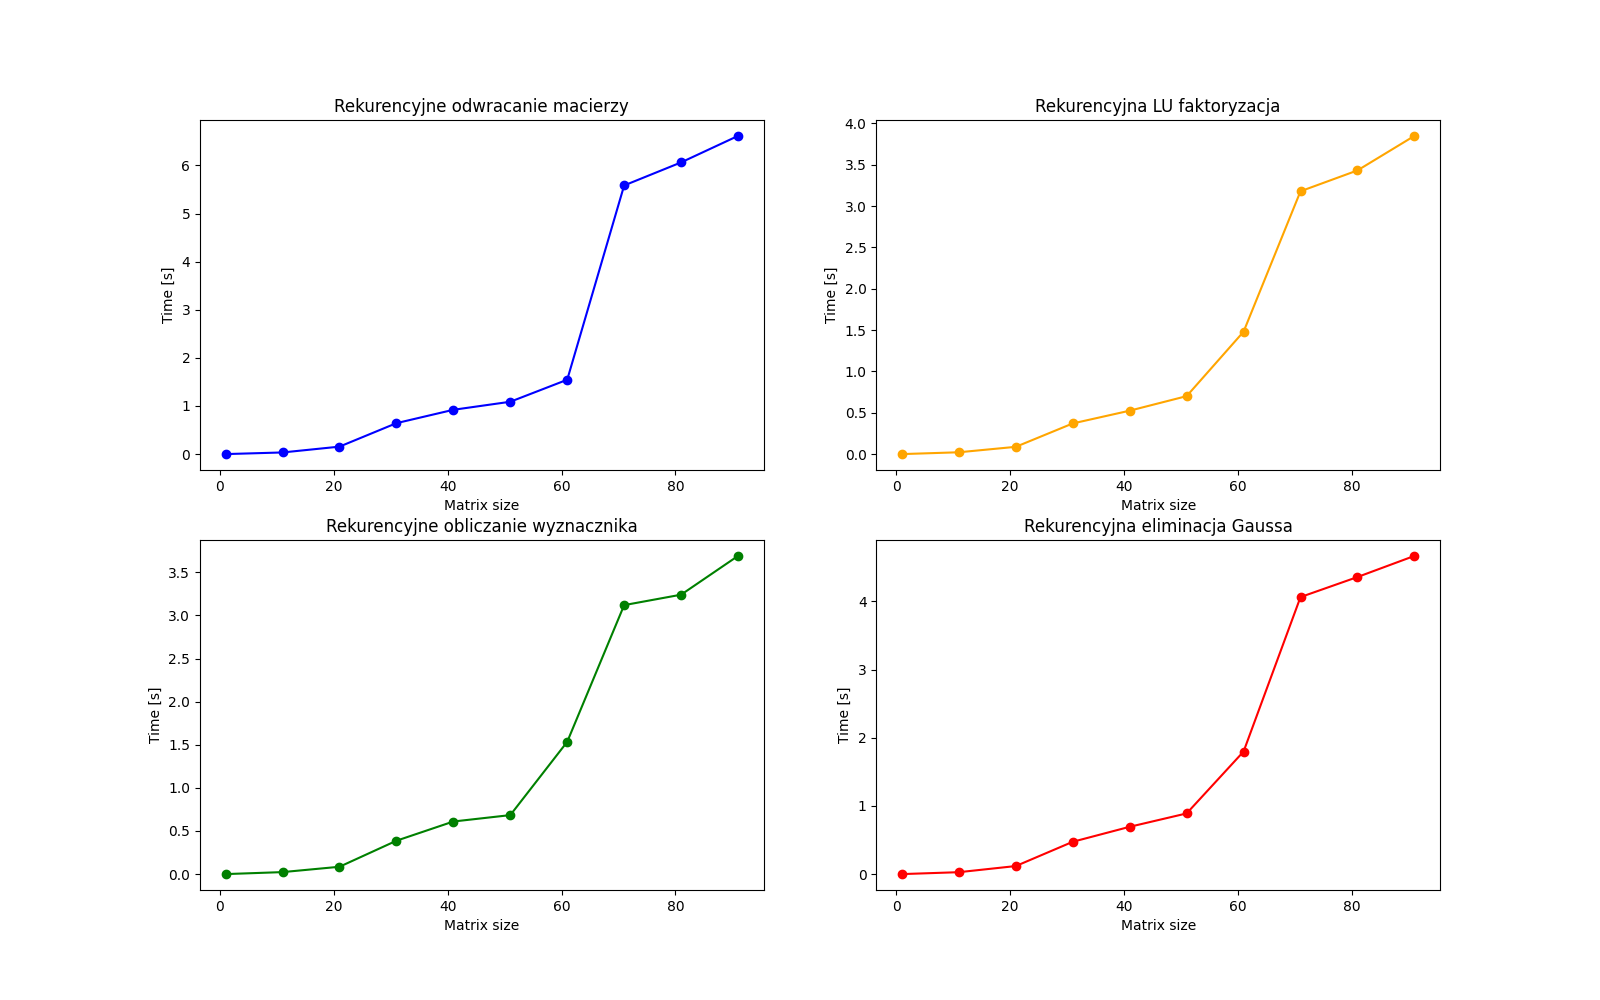
\includegraphics[width=0.8\linewidth]{zad2_time.png}
        \caption{Porównanie czasu działania każdego algorytmu.}
    \end{figure}

    \subsection{Liczba operacji zmienno-przecinkowych}
    \begin{figure}[H]
        \centering
        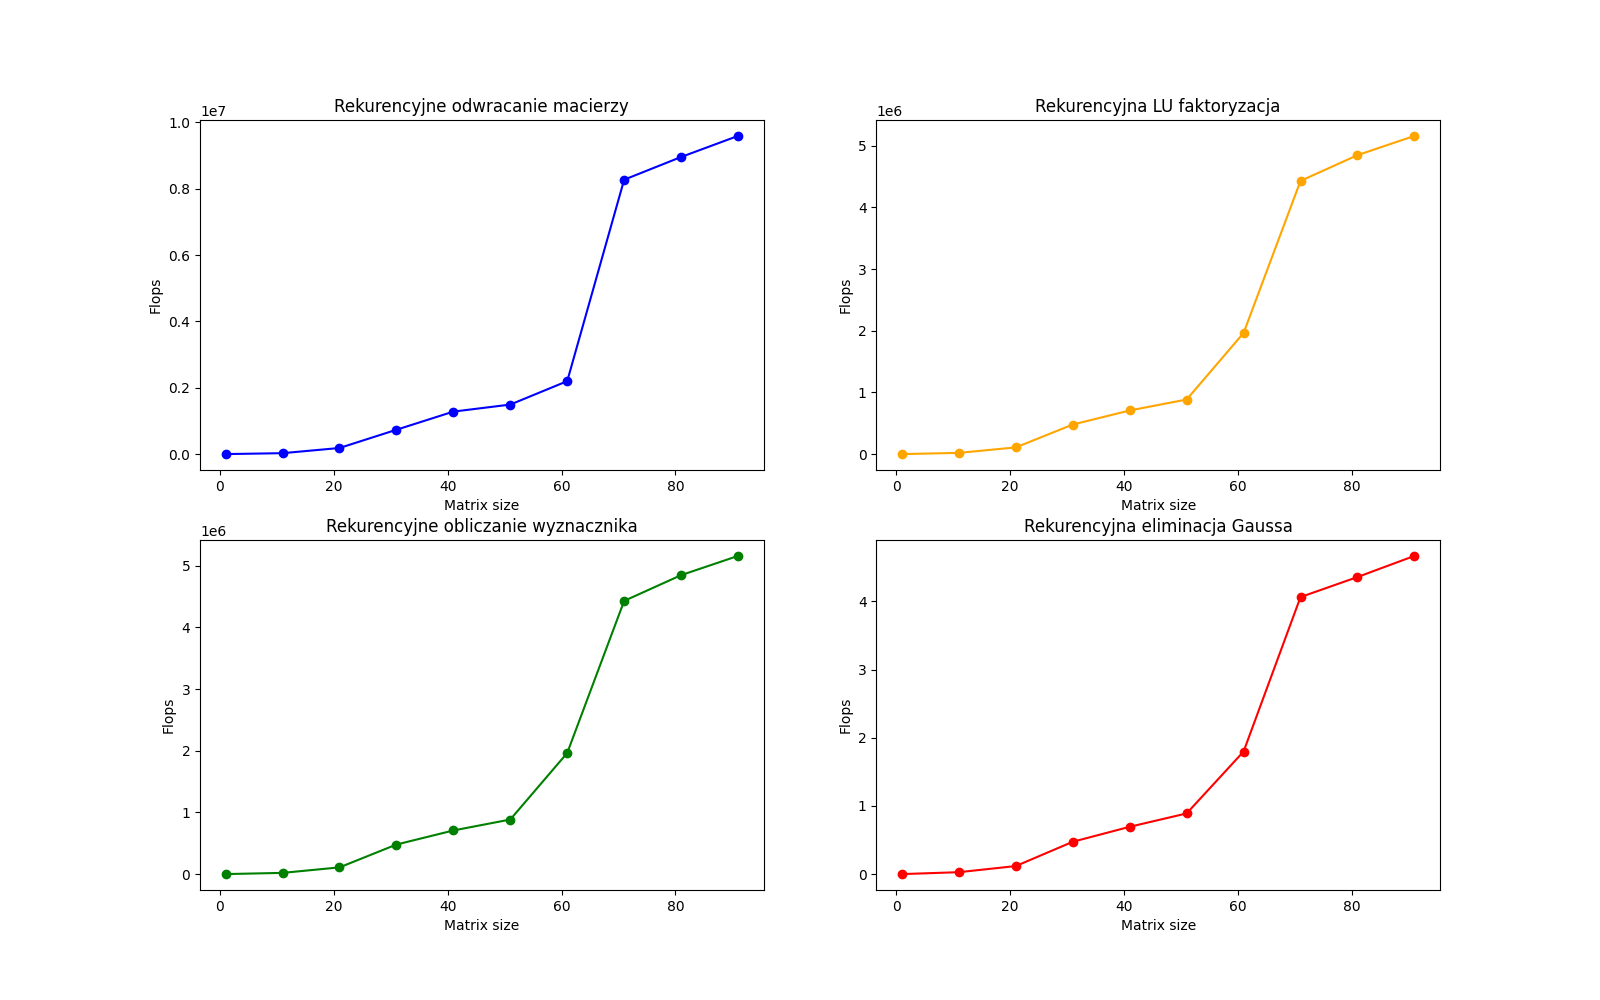
\includegraphics[width=0.8\linewidth]{zad2_flops.png}
        \caption{Porównanie liczby operacji zmienno-przecinkowych
            każdego algorytmu.}
    \end{figure}

    \section{Oszacowanie złożoności obliczeniowej}
    W przypadku każdego algorytmu zmierzony został czas obliczeń dla
    \[
        n \in [8,100]
    \]
    dla $40$ równoodległych od siebie wartości oraz dopasowana krzywa
    złożoności obliczeniowej metodą \texttt{curve\_fit} z pakietu
    \texttt{scipy.optimize}.

    \subsection{Rekurencyjne odwracanie macierzy}
    Dopasowana krzywa:
    \[
        y=3.7 \cdot 10^{-4} \cdot x^{2.12}
    \]
    Zatem oszacowana złożoność obliczeniowa wynosi:
    \[
        O(n)=n^{2.12}
    \]
    a teoretyczna złożoność:
    \[
        O(n)=n^{2.81}
    \]
    \begin{figure}[H]
        \centering
        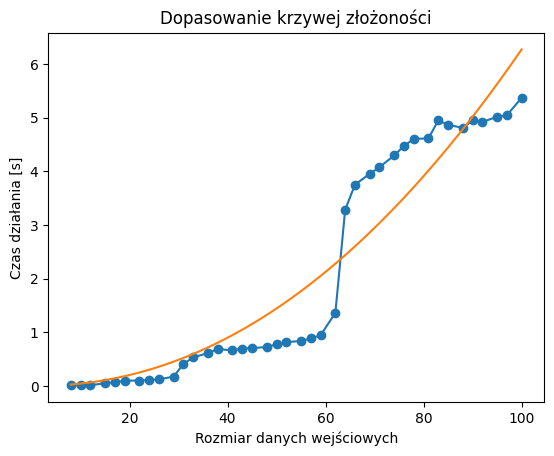
\includegraphics[width=0.7\linewidth]{zlozonosc_rek_mnozenie.png}
        \caption{Krzywa złożoności dla rekurencyjnego odwracania macierzy.}
    \end{figure}

    \subsection{Rekurencyjna LU faktoryzacja}
    Dopasowana krzywa:
    \[
        y=3 \cdot 10^{-4} \cdot x^{2.04}
    \]
    Zatem oszacowana złożoność obliczeniowa wynosi:
    \[
        O(n)=n^{2.04}
    \]
    a teoretyczna złożoność:
    \[
        O(n)=n^3
    \]
    \begin{figure}[H]
        \centering
        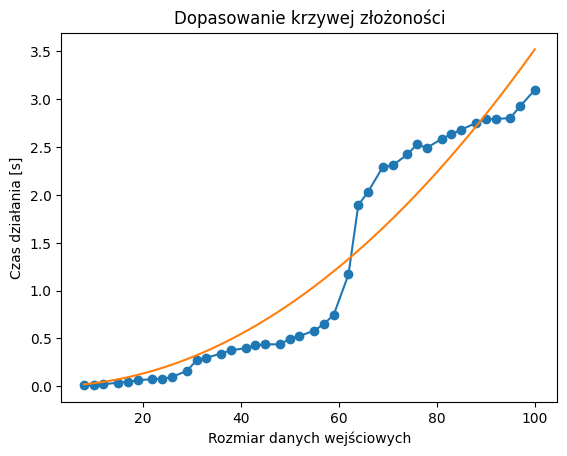
\includegraphics[width=0.7\linewidth]{zlozonosc_lu.png}
        \caption{Krzywa złożoności dla rekurencyjnej LU faktoryzacji.}
    \end{figure}

    \subsection{Rekurencyjne liczenie wyznacznika}
    Dopasowana krzywa:
    \[
        y=3.1 \cdot 10^{-4} \cdot x^{2.02}
    \]
    Zatem oszacowana złożoność obliczeniowa wynosi:
    \[
        O(n)=n^{2.02}
    \]
    a teoretyczna złożoność:
    \[
        O(n)=n^3
    \]
    \begin{figure}[H]
        \centering
        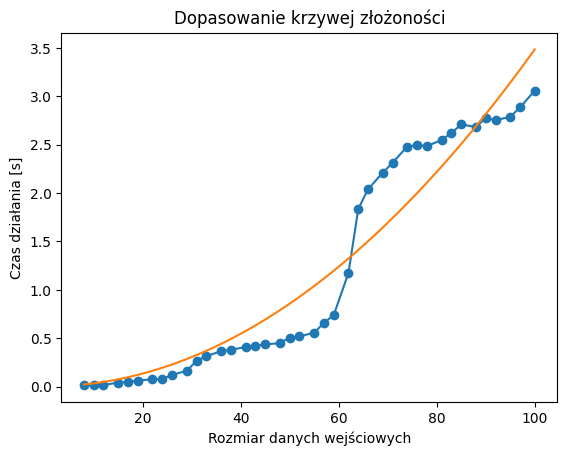
\includegraphics[width=0.7\linewidth]{zlozonosc_det.png}
        \caption{Krzywa złożoności dla rekurencyjnego liczenia
            wyznacznika macierzy.}
    \end{figure}

    \subsection{Rekurencyjna eliminacja Gaussa}
    Dopasowana krzywa:
    \[
        y=3.9 \cdot 10^{-4} \cdot x^{2.03}
    \]
    Zatem oszacowana złożoność obliczeniowa wynosi:
    \[
        O(n)=n^{2.03}
    \]
    a teoretyczna złożoność:
    \[
        O(n)=n^3
    \]
    \begin{figure}[H]
        \centering
        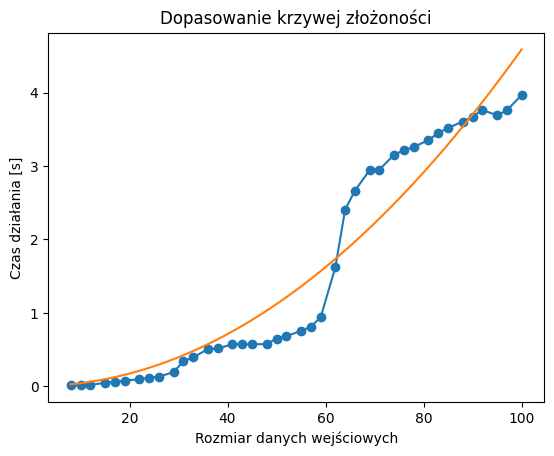
\includegraphics[width=0.7\linewidth]{zlozonosc_gauss.png}
        \caption{Krzywa złożoności dla rekurencyjnej eliminacji
            Gaussa.}
    \end{figure}

    \subsection{Podsumowanie}
    Oszacowane złożoności obliczeniowe prezentowanych algorytmów
    odbiegają od złożoności teoretycznych. Może być to spowodowane
    niewystarczająco stabilną platformą testową lub szeregiem
    usprawnień oferowanych przez biblioteki Pythona.

    \section{Porównanie obliczeń z biblioteką NumPy}
    
\end{document}
